%%%%%%%%%%%%%%%%%%%%%%%%%%%%%%%%%%%%%%%%%%%%%%%%%%%%%%%%%%%%%%%%%%%%%%%%%%%%%%%
\chapter{Bound on the Lipschitz Constant of Convolutional Layers}
\label{chapter:ch5-lipschitz_bound}
%%%%%%%%%%%%%%%%%%%%%%%%%%%%%%%%%%%%%%%%%%%%%%%%%%%%%%%%%%%%%%%%%%%%%%%%%%%%%%%
\localtoc


%%%%%%%%%%%%%%%%%%%%%%%%%%%%%%%%%%%%%%%%%%%%%%%%%%%%%%%%%%%%%%%%%%%%%%%%%%%%%%%
\section{Introduction}
\label{section:ch5-introduction}
%%%%%%%%%%%%%%%%%%%%%%%%%%%%%%%%%%%%%%%%%%%%%%%%%%%%%%%%%%%%%%%%%%%%%%%%%%%%%%%


The last few years have witnessed a growing interest in Lipschitz regularization of neural networks, with the aim of improving their generalization~\cite{bartlett2017spectrally}, their robustness to adversarial attacks~\cite{tsuzuku2018lipschitz, farnia2018generalizable}, or their generation abilities (\eg for GANs: \citet{miyato2018spectral,arjovsky2017wasserstein}).
Unfortunately computing  the exact Lipschitz constant of a neural network is NP-hard~\cite{scaman2018lipschitz} and in practice, existing techniques such as~\citet{scaman2018lipschitz}, \citet{fazlyab2019efficient} or~\citet{latorre2020lipschitz} are difficult to implement for neural networks with more than one or two layers, which hinders their use in deep learning applications.

To overcome this difficulty, most of the work has focused on computing the Lipschitz constant of \emph{individual layers} instead.
The product of the Lipschitz constant of each layer is an upper-bound for the Lipschitz constant of the entire network, and it can be used as a surrogate to perform Lipschitz regularization.
Since most common activation functions (such as ReLU) have a Lipschitz constant equal to one, the main bottleneck is to compute the Lipschitz constant of the underlying linear application which is equal to its largest singular value.
The work in this line of research mainly relies on the celebrated iterative algorithm by~\citet{golub2000eigenvalue} used to approximate the maximum singular value of a linear function.
Although generic and accurate, this technique is also computationally expensive, which impedes its usage in large training settings.

In this chapter we introduce a new upper bound on the largest singular value of convolution layers that is both tight and easy to compute.
Instead of using the power method to iteratively approximate this value, we rely on Toeplitz matrix theory and its links with Fourier analysis.
Our work is based on the result of~\citet{gray2006toeplitz} which states that an upper bound on the singular value of Toeplitz matrices can be computed from the inverse Fourier transform of the characteristic sequence of these matrices.
We first extend this result to doubly-block Toeplitz matrices (\ie, block Toeplitz matrices where each block is Toeplitz) and then to convolutional operators, which can be represented as stacked sequences of doubly-block Toeplitz matrices.
From our analysis immediately follows an algorithm for bounding the Lipschitz constant of a convolutional layer, and by extension the Lipschitz constant of the whole network.
We theoretically study the approximation of this algorithm and show experimentally that it is more efficient and accurate than competing approaches.

Finally, we illustrate our approach on adversarial robustness.
Recent work has shown that empirical methods such as adversarial training (AT) offer poor generalization~\cite{schmidt2018adversarially}, and can be improved by applying Lipschitz regularization~\cite{farnia2018generalizable}.
To illustrate the benefit of our new method, we train a large, state-of-the-art Wide ResNet architecture with Lipschitz regularization and show that it offers a significant improvement over adversarial training alone, and over other methods for Lipschitz regularization.
In summary, we make the three following contributions:
\begin{enumerate}
  \item We devise an upper bound on the singular values of the operator matrix of convolutional layers by leveraging Toeplitz matrix theory and its links with Fourier analysis.
  \item We propose an efficient algorithm to compute this upper bound which enables its use in the context of Convolutional Neural Networks.
  \item We use our method to regularize the Lipschitz constant of neural networks for adversarial robustness and show that it offers a significant improvement over AT alone.
\end{enumerate}


%%%%%%%%%%%%%%%%%%%%%%%%%%%%%%%%%%%%%%%%%%%%%%%%%%%%%%%%%%%%%%%%%%%%%%%%%%%%%%%
\section{Results on the Spectrum of Matrices from the Toeplitz Family}
\label{section:ch5-results_on_the_spectrum_of_matrices_from_the_toeplitz_family}
%%%%%%%%%%%%%%%%%%%%%%%%%%%%%%%%%%%%%%%%%%%%%%%%%%%%%%%%%%%%%%%%%%%%%%%%%%%%%%%

%%%%%%%%%%%%%%%%%%%%%%%%%%%%%%%%%%%%%%%%%%%%%%%%%%%%%%%%%%%%%%%%%%%%%%%%%%%%%%%
\subsection{Upper-Bounds on the Largest Singular Value of Toeplitz and Block Toeplitz Matrices}
\label{subsection:ch5-upper_bounds_on_the_largest_singular_value_of_toeplitz_and_block_toeplitz_matrices}
%%%%%%%%%%%%%%%%%%%%%%%%%%%%%%%%%%%%%%%%%%%%%%%%%%%%%%%%%%%%%%%%%%%%%%%%%%%%%%%

In order to devise a bound on the Lipschitz constant of a convolution layer as used by the Deep Learning community, we study the properties of \emph{doubly-block Toeplitz matrices}. 
Doubly-block Toeplitz matrices inherits the properties of Toeplitz and block Toeplitz matrices.
Recall that Toeplitz and block Toeplitz matrices do not have a closed-form expression of their eigenvalues as their circulant counterpart.
However, we can represent Toeplitz and block Toeplitz matrices with a 2$\pi$-periodic function which can describe very precisely the spectrum of the matrices. 
Let $\{a_h\}_{h \in \Iset_n}$ be the characteristic sequence of a Toeplitz matrix $\Amat \in \Rbb^{n \times n}$ and let $\{\Bmatsf{(h)}\}_{h \in \Iset_n}$ be the characteristic sequence of $m \times m$ blocks of a block Toeplitz matrix $\Bmat \in \Rbb^{nm \times nm}$.
The matrices are therefore denoted $\Amat = \leftmat a_{j-i} \rightmat_{i,j \in \Iset_n}$ and $\Bmat = ( \Bmatsf^{(j-i)} )_{i,j \in \Iset_n}$ where $\Iset_n = \left\{ -n+1, \cdots, n-1 \right\}$.
Building on the results presented in the Background (\Cref{chapter:ch2-background}), we can define trigonometric polynomials $f: \Rbb \rightarrow \Cbb$ and $F: \Rbb \rightarrow \Cbb^{m \times m}$ such that:
\begin{equation}
  f(\omega) = \sum_{h \in \Iset_n} a_h e^{\ci h \omega} \quad \quad  F(\omega) = \sum_{h \in \Iset_n} \Bmatsf^{(h)} e^{\ci h \omega}
\end{equation}
which are the \emph{inverse Fourier transforms} of the sequences $\{a_h\}_{h \in \Iset_n}$ and $\{\Bmatsf^{(h)}\}_{h \in \Iset_n}$.
From there, similarly to the work done by~\citet{grenander1958toeplitz}, we define an operator $\Tmat$ mapping integrable functions to Toeplitz matrices:
\begin{equation} \label{equation:expression_toeplitz_matrix}
  \Tmat(g) \triangleq\leftmat\frac{1}{2\pi}\int_{0}^{2\pi}e^{-\ci(i-j)\omega}g(\omega)\,d\omega\rightmat_{i,j \in \Iset^+_n} \enspace,
\end{equation}
such that $\Tmat(f) = \Amat$ and $\Tmat(F) = \Bmat$.


Now, we can state two known theorems which upper bound the largest singular value of Toeplitz and block Toeplitz matrices with respect to their generating functions.
\begin{theorem}[Bound on the singular values of Toeplitz matrices] \label{theorem:teoplitz_sup_singular}
  Let $f: \Rbb \rightarrow \Cbb$, be continuous and $2\pi$-periodic. Let $\Tmat(f) \in \Rbb^{n \times n}$ be a Toeplitz matrix generated by the function $f$, then:
  \begin{align}
    \sigma_1 \left( \Tmat(f) \right) \leq \sup_{\omega \in [0, 2\pi]} |f(\omega)|.
  \end{align}
  \removespace
\end{theorem}
\noindent
\Cref{theorem:teoplitz_sup_singular} is a direct application of  Lemma 4.1 by~\citet{gray2006toeplitz} for real Toeplitz matrices. 

\begin{theorem}[Bound on the singular values of Block Toeplitz matrices ~\citet{gutierrez2012block}] \label{theorem:block_teoplitz_sup_singular}
  Let $F: \Rbb \rightarrow \Cbb^{m \times m}$ be a matrix-valued function which is continuous and $2 \pi$-periodic.
  Let $\Tmat(F) \in \Rbb^{mn \times mn}$ be a block Toeplitz matrix generated by the function $F$, then:
  \begin{align}
    \sigma_1 \left( \Tmat(F) \right) \leq \sup_{\omega \in [0, 2\pi]} \sigma_1 \left( F\left( \omega \right) \right) .
  \end{align}
  \removespace
\end{theorem}





%%%%%%%%%%%%%%%%%%%%%%%%%%%%%%%%%%%%%%%%%%%%%%%%%%%%%%%%%%%%%%%%%%%%%%%%%%%%%%%%
\subsection{Upper-Bound on the Largest Singular Value of Doubly-Block Toeplitz Matrices}
\label{subsection:ch5-bound_on_the_singular_value_of_doubly-block_toeplitz_matrices}
%%%%%%%%%%%%%%%%%%%%%%%%%%%%%%%%%%%%%%%%%%%%%%%%%%%%%%%%%%%%%%%%%%%%%%%%%%%%%%%%

We extend the reasoning from Toeplitz and block Toeplitz matrices to doubly-block Toeplitz matrices (\ie block Toeplitz matrices where each block is also a Toeplitz matrix).
A doubly-block Toeplitz matrix can be generated by a function $f: \Rbb^2 \rightarrow \Cbb$ using the 2-dimensional inverse Fourier transform.
For this purpose, we define an operator $\Dmat$ which maps a function $f: \Rbb^2 \rightarrow \Cbb$ to a doubly-block Toeplitz matrix of size $nm \times nm$.
For the sake of clarity, the dependence of $\Dmat(f)$ on $m$ and $n$ is omitted.
Let $\Dmat(f) = \leftmat \Dmat_{i,j}(f)\rightmat_{i,j \in \Iset^+_n}$ where $\Dmat_{i,j}(f)$ is a $m \times m$ matrix defined as:
\begin{equation} \label{equation:doubly_block_toeplitz_operator}
  \Dmat_{i,j}(f) = \leftmat \frac{1}{4\pi^{2}} \int_{[0,2\pi]^{2}} e^{- \ci \left((i-j)\omega_{1}+(k-l)\omega_{2}\right)}f(\omega_{1},\omega_{2})\,d(\omega_{1},\omega_{2}) \rightmat_{k,l \in \Iset^+_m} \enspace.
\end{equation}

We are now able to combine \Cref{theorem:teoplitz_sup_singular,theorem:block_teoplitz_sup_singular} to bound the largest singular value of doubly-block Toeplitz matrices with respect to their generating functions. 
Note that in the following, we only consider generating functions as trigonometric polynomials with real coefficients therefore the matrices generated by $\Dmat(f)$ are real. We can now combine \Cref{theorem:teoplitz_sup_singular,theorem:block_teoplitz_sup_singular} to bound the largest singular value of a doubly-block Toeplitz Matrix. 

\begin{maintheorem}[Bound on the largest singular value of a Doubly-Block Toeplitz Matrix] \label{theorem:doubly_block_teoplitz_sup_singular}
  Let $f: \Rbb^2 \rightarrow \Cbb$ be a multivariate trigonometric polynomial of the form:
  \begin{equation}\label{equation:muli_variate_poly_on_M}
    f(\omega_1, \omega_2) \triangleq \sum_{h_1 \in \Iset_n} \sum_{h_2 \in \Iset_m} d_{h_1, h_2} e^{\ci (h_1 \omega_1 + h_2 \omega_2)}.
  \end{equation}
  Let $\Dmat$ the doubly-block Toeplitz operator such that $\Dmat(f) \in \Rbb^{nm \times nm}$ and where $d_{h_{1},h_{2}}$ is the ${h_2}^\textrm{th}$ scalar of the ${h_1}^\textrm{th}$ block of the doubly-Toeplitz matrix $\Dmat(f)$.
  Then, we have:
  \begin{align}
    \sigma_{1} \left( \Dmat(f) \right) &\leq \sup_{\omega_1, \omega_2 \in [0, 2\pi]^2}|f(\omega_1,\omega_2)|
  \end{align}
  \removespace
\end{maintheorem}


% Let $\Dmat(f) \in \Rbb^{nm \times nm}$ be a doubly-block Toeplitz matrix generated by the function $f$, then:
% where the function $f: \Rbb^2 \rightarrow \Cbb$, is a multivariate trigonometric polynomial of the form:
%
% where $d_{h_{1},h_{2}}$ is the ${h_2}^\textrm{th}$ scalar of the ${h_1}^\textrm{th}$ block of the doubly-Toeplitz matrix $\Dmat(f)$.



\begin{proof}[\Cref{theorem:doubly_block_teoplitz_sup_singular}]
  A doubly-block Toeplitz matrix is by definition a block matrix where each block is a Toeplitz matrix.
  We can then express a doubly-block Toeplitz matrix with the operator $\Tmat(F)$ where the matrix-valued generating function $F$ has Toeplitz coefficient.
  Let us define a matrix-valued trigonometric polynomial $F:\Rbb\rightarrow\Cbb^{n \times n}$ of the form:
  \begin{equation}
    F(\omega_1) = \sum_{h_1 \in N} \Amatsf^{(h_1)} e^{\ci h_1\omega_1}
  \end{equation}
  where $\Amatsf^{(h_1)}$ are Toeplitz matrices of size $m \times m$ determined by the sequence $\{d_{h_1, -m+1}, \dots, d_{h_1, m-1} \}$. 
  From \Cref{theorem:block_teoplitz_sup_singular} we have:
  \begin{equation}
  \sigma_1\left(\Tmat(F) \right) \leq \sup_{\omega_1 \in [0,2\pi] } \sigma_{1}\left( F(\omega_1) \right) \label{equation:th_bound_block_toeplitz}
  \end{equation}

  Because Toeplitz matrices are closed under addition and scalar product, $F(\omega_1)$ is also a Toeplitz matrix of size $m \times m$. 
  We can thus define a function $f:\Rbb^{2} \rightarrow \Cbb$ of the form 
  \begin{equation}
    f(\omega_1,\omega_2) = \sum_{h_1 \in N} \sum_{h_2 \in M} d_{h_1, h_2} e^{\ci \left( h_1\omega_1 + h_2 \omega_2\right)} \enspace,
  \end{equation}
  and such that $f(\omega_1,\ \cdot\ )$ is the generating function of $F(\omega_1)$.
  From \Cref{theorem:teoplitz_sup_singular}, we can write:
  \begin{align}
      \sigma_{1}\left( F(\omega_1) \right) &\leq \sup_{\omega_2 \in [0,2\pi]} \left| f(\omega_1, \omega_2) \right| \\
      \Leftrightarrow \sup_{\omega_1 \in [0,2\pi]} \sigma_{1}\left( F(\omega_1) \right) &\leq  \sup_{\omega_1, \omega_2 \in [0,2\pi]^2} \left| f(\omega_1, \omega_2) \right| \\
      \Leftrightarrow \sigma_1\left(\Tmat(F) \right) &\leq \sup_{\omega_1, \omega_2 \in [0,2\pi]^2} \left| f(\omega_1, \omega_2) \right|
  \end{align}
  Because the function $f(\omega_1,\ \cdot\ )$ is the generating function of $F(\omega_1)$ is it easy to show that the function $f$ is also the generating function of the matrix $\Tmat(F)$. Therefore, $\Tmat(F) = \Dmat(f)$ which concludes the proof. 
\end{proof}


%%%%%%%%%%%%%%%%%%%%%%%%%%%%%%%%%%%%%%%%%%%%%%%%%%%%%%%%%%%%%%%%%%%%%%%%%%%%%%%
\section{Extending the Bound to Convolutional Layers}
\label{section:ch5-bound_on_the_singular_values_of_convolutional_layers}
%%%%%%%%%%%%%%%%%%%%%%%%%%%%%%%%%%%%%%%%%%%%%%%%%%%%%%%%%%%%%%%%%%%%%%%%%%%%%%%

From now on, without loss of generality, we will assume that $n=m$ to simplify notations.
A discrete convolution operation with a 2-dimensional kernel applied on a 2-dimensional signal is equivalent to a matrix multiplication with a doubly-block Toeplitz matrix~\cite{jain1989fundamentals}.
However, in practice, the signal is most of the time 3-dimensional (RGB images for instance).
We call the channels of a signal \emph{channels in} denoted $\cin$.
The input signal is then of size $\cin \times n \times n$.
Furthermore, we perform multiple convolutions of the same signal which corresponds to the number of channels the output will have after the operation.
We call the channels of the output signal \emph{channels out} denoted $\cout$.
Therefore, the kernel is defined as a 4-dimensional tensor of size: $\cout \times \cin \times s \times s$. 

The operation performed by a 4-dimensional kernel on a 3-dimensional signal can be expressed by the concatenation (horizontally and vertically) of doubly-block Toeplitz matrices.
Hereafter, we bound the singular value of multiple vertically stacked doubly-block Toeplitz matrices which corresponds to the operation performed by a 3-dimensional kernel with $\cout = 1$ on a 3-dimensional signal.

\begin{theorem}[Bound on the largest singular value of stacked Doubly-block Toeplitz matrices] \label{theorem:bound_sv_stacked_dbt} 
  Consider doubly-block Toeplitz matrices $\Dmat(f_1), \dots, \Dmat(f_{\cin})$ where each $f_i: \Rbb^2 \rightarrow \Cbb$ is a multivariate polynomial of the same form as \Cref{equation:muli_variate_poly_on_M}.
  Construct a matrix $\Mmat$ with $\cin\times n^2$ rows and $n^2$ columns, as follows:
  \begin{equation}
    \Mmat \triangleq \leftmat \Dmat^\top(f_1), \dots, \Dmat^\top(f_{\cin}) \rightmat^\top .
  \end{equation}
  Then, we have:
  \begin{align} \label{equation:bound_asymptotic_equiv}
    \sigma_1 \left( \Mmat \right) &\leq \sup_{\omega_1, \omega_2 \in \left[0, 2\pi\right]^2} \sqrt{ \sum_{i=1}^{\cin} \left|f_i\right (\omega_1, \omega_2)|^2} \enspace.
  \end{align}
\end{theorem}

\noindent
In order to prove \Cref{theorem:bound_sv_stacked_dbt}, we will need the following lemmas:

\begin{lemma}[\citet{gutierrez2012block}] \label{theorem:properties_block_toeplitz}
  Let $f:\Rbb^2 \rightarrow \Cbb$ and $g:\Rbb^2 \rightarrow \Cbb$ be two continuous and $2\pi$-periodic functions. Let $\Dmat(f)$ and $\Dmat(g)$ be doubly-block Toeplitz matrices generated by the function $f$ and $g$ respectively. Then:
  \begin{itemize}
      \item $\Dmat^\top(f) = \Dmat(f^*)$
      \item $\Dmat(f) + \Dmat(g) = \Dmat(f + g)$
  \end{itemize}
  \removespace
\end{lemma}

\begin{lemma}[\citet{serra1994preconditioning}] \label{theorem:block_toeplitz_hermitian}
  If the doubly-block Toeplitz matrix $\Dmat(f)$ is generated by a function $f: \Rbb^2 \rightarrow \Rbb$, then the matrix $\Dmat(f)$ is Hermitian. 
\end{lemma}

\begin{lemma}[\citet{serra1994preconditioning}] \label{theorem:block_toeplitz_positive_definite}
  If the doubly-block Toeplitz matrix $\Dmat(f)$ is generated by a non-negative function $f$ not identically zero, then the matrix $\Dmat(f)$ is positive definite. 
\end{lemma}

\begin{lemma}[\citet{zhang2011matrix}] \label{theorem:diff_positive_semidefinite_matrices}
Let $\Amat$ and $\Bmat$ be Hermitian positive semi-definite matrices. If $\Amat - \Bmat$ is positive semi-definite, then:
  \begin{equation}
      \lambda_1 \left( \Bmat \right) \leq \lambda_1 \left( \Amat \right)
  \end{equation}
  \removespace
\end{lemma}


Before proving \Cref{theorem:bound_sv_stacked_dbt}, we generalize the famous Widom identity \cite{widom1976asymptotic} that expresses the relation between Toeplitz and Hankel matrices to doubly-block Toeplitz and Hankel matrices.
We will need to generalize the doubly-block Toeplitz operator presented in~\Cref{subsection:ch5-bound_on_the_singular_value_of_doubly-block_toeplitz_matrices}.

Let $\Gmat^{\alpha_p} (f) = \leftmat \Gmat^{\alpha_p}_{i,j}(f) \rightmat_{i,j \in \Iset^+_n}$ where $\Gmat^{\alpha_p}_{i,j}$ is defined as:
\begin{equation}
  \Gmat^{\alpha_p}_{i,j}(f) =\leftmat \frac{1}{4\pi^{2}}\int_{[0,2\pi]^{2}} e^{-\ci \alpha_p(i, j, k, l, \omega_1, \omega_2)}  f(\omega_{1},\omega_{2})\,d(\omega_{1},\omega_{2})
  \rightmat_{k,l \in \Iset^+_n} \enspace.
\end{equation}
Note that as with the operator $\Dmat(f)$ we only consider generating functions as trigonometric polynomials with real coefficients therefore the matrices generated by $\Gmat(f)$ are real. 
And as with the operator $\Dmat(f)$, the matrices generated by the operator $\Gmat^{\alpha_p}$ are of size $n^2 \times n^2$. 

\noindent
We will use the following $\alpha$ functions:
\begin{itemize}
    \item[] $\alpha_0(i, j, k, l, \omega_1, \omega_2) = (-j-i-1)\omega_1 + (k-l)\omega_2$
    \item[] $\alpha_1(i, j, k, l, \omega_1, \omega_2) = (i-j)\omega_1 + (-l-k-1)\omega_2$
    \item[] $\alpha_2(i, j, k, l, \omega_1, \omega_2) = (-j-i-1)\omega_1 + (-l-k-1)\omega_2$
    \item[] $\alpha_3(i, j, k, l, \omega_1, \omega_2) = (-j-i+n)\omega_1 + (-l-k-1)\omega_2$
\end{itemize}

\noindent
We now present the generalization of the Widom identity for Doubly-Block Toeplitz matrices below:
\begin{lemma}[Generalization of Widom Identity] \label{lemma:ch5-widom_idenity}
  Let $f:\Rbb^2 \rightarrow \Cbb$ and $g:\Rbb^2 \rightarrow \Cbb$ be two continuous and $2\pi$-periodic functions. 
  We can decompose the Doubly-Block Toeplitz matrix $\Dmat(fg)$ as follows:
  \begin{equation}
      \Dmat(fg) = \Dmat(f)\Dmat(g) + \sum_{p=0}^3 \Gmat^{\alpha_p \top}(f^*) \Gmat^{\alpha_p}(g) + \Jmat \left( \sum_{p=0}^3 \Gmat^{\alpha_p \top}(f) \Gmat^{\alpha_p }(g^*) \right) \Jmat.
  \end{equation}
  where $\Jmat$ is the reflection of the identity matrix of size $n^2 \times n^2$.
\end{lemma}

\noindent
The proof of this Lemma is available in Appendix~\ref{appendix:ap1-proof_of_the_generalization_of_widom_identity}.
Now we have all the element to prove \Cref{theorem:bound_sv_stacked_dbt} which bounds the largest singular value of vertically stacked doubly-block Toeplitz matrices with their generating functions. 

\begingroup
\addtolength{\jot}{1.5em}

\begin{proof}[\Cref{theorem:bound_sv_stacked_dbt}]
First, let us observe the following:
\begin{equation}
    \sigma_1^2 \left( \Mmat \right) = \lambda_1 \left( \Mmat^{\top} \Mmat \right) = \lambda_1 \left( \sum_{i=1}^{\cin} \Dmat^{\top} \left(f_i \right) \Dmat (f_i) \right).
\end{equation}

And the fact that:
\begin{align}
    \lambda_1 \left( \sum_{i=1}^{\cin} \Dmat \left(|f_i|^2 \right) \right) \quad &\stackrel{\text{by \Cref{theorem:properties_block_toeplitz}}}{=} \quad \lambda_1 \left( \Dmat \left( \sum_{i=1}^{\cin} |f_i|^2 \right) \right) \\ 
    \quad &\stackrel{\text{by \Cref{theorem:block_toeplitz_hermitian}}}{=} \quad \sigma_1 \left( \Dmat \left( \sum_{i=1}^{\cin} |f_i|^2 \right) \right) \\
    \quad &\stackrel{\text{by \Cref{theorem:doubly_block_teoplitz_sup_singular}}}{\leq} \quad \sup_{\omega_1, \omega_2 \in [0, 2\pi]^2} \sum_{i=1}^{\cin} |f_i(\omega_1, \omega_2)|^2.
\end{align}

\noindent
To prove the Theorem, we simply need to demonstrate that the following inequality holds:
\begin{equation} \label{equation:eq2}
    \lambda_1 \left( \sum_{i=1}^{\cin} \Dmat^{\top} \left(f_i \right) \Dmat (f_i) \right) \leq \lambda_1 \left( \Dmat \left( \sum_{i=1}^{\cin} |f_i|^2 \right) \right). 
\end{equation}

\noindent
From the positive definiteness of the following matrix:
\begin{equation}
    \Dmat \left( \sum_{i=1}^{\cin} |f_i|^2 \right) - \sum_{i=1}^{\ci} \Dmat^{\top} \left(f_i \right) \Dmat (f_i),
\end{equation}

\noindent
One can observe that the r.h.s is a real symmetric positive definite matrix by \Cref{theorem:block_toeplitz_positive_definite,theorem:block_toeplitz_hermitian}. Furthermore, the l.h.s is a sum of positive semi-definite matrices. Therefore, if the subtraction of the two is positive semi-definite, one could apply \Cref{theorem:diff_positive_semidefinite_matrices} to prove the \Cref{equation:eq2}. 
We know from \Cref{lemma:ch5-widom_idenity} that 
\begin{equation}
    \Dmat(fg) - \Dmat(f)\Dmat(g) = \sum_{p=0}^3 \Gmat^{\alpha_p \top}(f^*) \Gmat^{\alpha_p}(g) + \Jmat \left( \sum_{p=0}^3 \Gmat^{\alpha_p \top}(f) \Gmat^{\alpha_p}(g^*) \right) \Jmat.
\end{equation}
By choosing $f = f^*$, $g = f$ and with the use of \Cref{theorem:properties_block_toeplitz}, we obtain:
\begin{align} \label{equation:widom_identity_block_topelitz}
  \Dmat(f^* f) - \Dmat(f^*)\Dmat(f)
  &= \Dmat(|f|^2) - \Dmat^{\top}(f)\Dmat(f) \\
  &= \sum_{p=0}^3 \Gmat^{\alpha_p \top}(f)\Gmat^{\alpha_p}(f) + \Jmat \left( \sum_{p=0}^3 \Gmat^{\alpha_p \top}(f^*)\Gmat^{\alpha_p} (f^*) \right) \Jmat .
\end{align}

\noindent
From \Cref{equation:widom_identity_block_topelitz}, we can see that the matrix $\Dmat(|f|^2) - \Dmat^{\top}(f)\Dmat(f)$
is positive semi-definite because it can be decomposed into a sum of positive semi-definite matrices and because positive semi-definiteness is closed under addition, we have:

\begin{align}
    \sum_{i=1}^{\cin} \leftmat \Dmat \left( |f_i|^2 \right) - \Dmat^{\top} \left(f_i \right) \Dmat (f_i) \rightmat &\geq 0
\end{align}

\noindent
By re-arranging and with the use \Cref{theorem:properties_block_toeplitz}, we obtain:
\begin{align}
   \sum_{i=1}^{\cin} \leftmat \Dmat \left( |f_i|^2 \right) \rightmat - \sum_{i=1}^{\cin} \leftmat \Dmat^{\top} \left(f_i \right) \Dmat (f_i) \rightmat &\geq 0 \\
    \Dmat \left( \sum_{i=1}^{\cin} |f_i|^2 \right) - \sum_{i=1}^{\cin} \leftmat \Dmat^{\top} \left(f_i \right) \Dmat (f_i) \rightmat &\geq 0
\end{align}

\noindent
We can conclude that the \Cref{equation:eq2} is true and therefore by \Cref{theorem:diff_positive_semidefinite_matrices} we have:
\begin{align}
  \lambda_1 \left( \sum_{i=1}^{\cin} \Dmat^{\top} \left(f_i \right) \Dmat (f_i) \right) &\leq \lambda_1 \left( \Dmat \left( \sum_{i=1}^{\cin} |f_i|^2 \right) \right) \\
  \Leftrightarrow \sigma_1^2 \left( \Mmat \right) &\leq \sup_{\omega_1, \omega_2 \in [0, 2\pi]^2} \sum_{i=1}^{\cin} |f_i(\omega_1, \omega_2)|^2 \\
  \Leftrightarrow \sigma_1 \left( \Mmat \right) &\leq \sup_{\omega_1, \omega_2 \in [0, 2\pi]^2} \sqrt{ \sum_{i=1}^{\cin} |f_i(\omega_1, \omega_2)|^2 }
\end{align}
which concludes the proof. 
\end{proof}

\endgroup

\pagebreak

To have a bound on the full convolution operation, we extend \Cref{theorem:bound_sv_stacked_dbt} to take into account the number of output channels.
The matrix of a full convolution operation is a block matrix where each block is a doubly-block Toeplitz matrix.
Below, we present our main result:

\begin{maintheorem}[Bound on the largest singular value on the convolution operation] \label{theorem:ch5-bound_max_sv_convolution} 
  Let us define doubly-block Toeplitz matrices $\Dmat(f_{1, 1}), \dots, \Dmat(f_{\cin, \cout})$ where each $f_{i,j}: \Rbb^2 \rightarrow \Cbb$ is a multivariate polynomial of the same form as \Cref{equation:muli_variate_poly_on_M}.
  Construct a matrix $\Mmat$ with $\cin\times n^2$ rows and $\cout\times n^2$ columns such as
  Then, we have:
  \begin{equation} \label{equation:lipbound_sv}
     \sigma_1 \left( \Mmat \right) \leq \sqrt{ \sum_{i=1}^{\cout} \sup_{\omega_1, \omega_2 \in [0, 2\pi]^2} \sum_{j = 1}^{\cin} \left|f_{ij}(\omega_1, \omega_2) \right|^2 } .
  \end{equation} 
\end{maintheorem}

First, in order to prove \Cref{theorem:ch5-bound_max_sv_convolution}, we will need the following lemma which bound the singular values of a matrix constructed from the concatenation of multiple matrices.
\begin{lemma}[Bound on the singular values of concatenation of matrices] \label{theorem:ch2-bound_concatenation_matrices}
  Let us define matrices $\Amat^{(1)}, \dots, \Amat^{(p)}$ with $\Amat^{(i)} \in \Rbb^{n \times n}$. Let us construct the matrix $\Mmat \in \Rbb^{n \times pn}$ as follows:
  \begin{equation}
    \Mmat \triangleq \leftmat \Amat^{(1)}, \dots, \Amat^{(p)} \rightmat
  \end{equation}
  where $\leftmat\ \cdot\ \rightmat$ define the concatenation operation. Then, we can bound the singular values of the matrix $\Mmat$ as follows:
  \begin{equation}
    \sigma_1(\Mmat) \leq \sqrt{\sum_{i=1}^p \sigma_1(\Amat^{(i)})^2}
  \end{equation}
\end{lemma}

\begingroup
\allowdisplaybreaks
\addtolength{\jot}{1.5em}

\begin{proof}[\Cref{theorem:ch2-bound_concatenation_matrices}]
  \begin{align}
    \sigma_1\left(\Mmat\right)^2 &= \lambda_1\left(\Mmat \Mmat^\top\right) \\
    &= \lambda_1\left( \sum_{i=1}^p\Amat^{(i)} \Amat^{(i)\top}  \right) \\
    &\leq \sum_{i=1}^p \lambda_1\left( \Amat^{(i)} \Amat^{(i)\top}  \right) \\
    &\leq \sum_{i=1}^p \sigma_1\left( \Amat^{(i)} \right)^2 \\
    \Leftrightarrow \sigma_1\left(\Mmat\right) &\leq \sqrt{\sum_{i=1}^p \sigma_1(\Amat^{(i)})^2}
  \end{align}
  which concludes the proof.
\end{proof}

\noindent
Now, the proof of \Cref{theorem:ch5-bound_max_sv_convolution} is a simple combination of \Cref{theorem:ch2-bound_concatenation_matrices} and \Cref{theorem:bound_sv_stacked_dbt}.

\begin{proof}[\Cref{theorem:ch5-bound_max_sv_convolution}]
  Let us define the matrix $\Mmat^{(i)}$ as follows:
\begin{equation}
  \Mmat^{(i)} = \leftmat \Dmat(f_{1, i})^\top, \dots, \Dmat(f_{\cin, i})^\top \rightmat^\top .
\end{equation}
We can express the matrix $\Mmat$ as the concatenation of multiple $\Mmat^{(i)}$ matrices:
\begin{equation}
  \Mmat = \leftmat \Mmat^{(1)}, \dots, \Mmat^{(\cout)} \rightmat
\end{equation}
Then, we can bound the singular values of the matrix $\Mmat$ as follows:
\begin{align}
  \sigma_1\left(\Mmat\right) &\stackrel{\text{by \Cref{theorem:ch2-bound_concatenation_matrices}}}{\leq} \sqrt{\sum_{i=1}^{\cout} \sigma_1(\Mmat^{(i)})^2} \\
  \sigma_1\left(\Mmat\right) &\stackrel{\text{by \Cref{theorem:bound_sv_stacked_dbt}}}{\leq} \sqrt{\sum_{j=1}^{\cout} \sup_{\omega_1, \omega_2 \in [0, 2\pi]^2} \sum_{i=1}^{\cin} |f_{i,j}(\omega_1, \omega_2)|^2 }
\end{align}
which concludes the proof. 
\end{proof}

\endgroup
\pagebreak

\Cref{theorem:ch5-bound_max_sv_convolution} depends on the convolution matrix $\Mmat$, however, we can easily formulate the bound with the values of a 4-dimensional kernel.
Let us define a kernel $\Kmat \in \Rbb^{\cout \times \cin \times s \times s}$, a padding $p \in \Nbb$ and $d = \lfloor s / 2 \rfloor$ the degree of the trigonometric polynomial, then:
\begin{equation}
  f_{ij}(\omega_1, \omega_2) = \sum_{h_1 = -d}^d \sum_{h_2 = -d}^d k_{i, j, h_1,h_2} e^{\ci (h_1 \omega_1 + h_2 \omega_2)}.
\end{equation}
where $k_{i, j, h_1,h_2} = \leftmat \Kmat \rightmat_{i, j, a, b}$ with $a =  s - p - 1 + i$ and $b =  s - p - 1 + j$.

In the rest of the chapter, we will refer to the bound in \Cref{theorem:ch5-bound_max_sv_convolution} applied to a kernel as $\lipbound$ and we denote $\lipbound(\Kmat)$ the Lipschitz upper bound of the convolution performed by the kernel $\Kmat$. 


%%%%%%%%%%%%%%%%%%%%%%%%%%%%%%%%%%%%%%%%%%%%%%%%%%%%%%%%%%%%%%%%%%%%%%%%%%%%%%%
\section{Computation and Performance Analysis of LipBound}
\label{section:ch5-computation_and_performance_analysis_of_lipbound}
%%%%%%%%%%%%%%%%%%%%%%%%%%%%%%%%%%%%%%%%%%%%%%%%%%%%%%%%%%%%%%%%%%%%%%%%%%%%%%%

This section aims at analyzing the bound introduced in \Cref{theorem:ch5-bound_max_sv_convolution}.
First, we present an algorithm to efficiently compute the bound, we analyze its tightness by comparing it against the true largest singular value.
Finally, we compare the efficiency and the accuracy of our bound against the state-of-the-art. 

%%%%%%%%%%%%%%%%%%%%%%%%%%%%%%%%%%%%%%%%%%%%%%%%%%%%%%%%%%%%%%%%%%%%%%%%%%%%%%%%
\subsection{The Maximum Modulus of a Trigonometric Polynomial}
\label{subsection:ch5-computing_the_maximum_modulus_of_a_trigonometric_polynomial}
%%%%%%%%%%%%%%%%%%%%%%%%%%%%%%%%%%%%%%%%%%%%%%%%%%%%%%%%%%%%%%%%%%%%%%%%%%%%%%%%

In order to compute $\lipbound$ from \Cref{theorem:ch5-bound_max_sv_convolution}, we have to compute the maximum modulus of several trigonometric polynomials.
However, finding the maximum modulus of a trigonometric polynomial has been known to be NP-Hard~\cite{pfister2018bounding}, and in practice they exhibit low convexity (see \Cref{figure:contour_plot_trigonometric_polynomials}).
We found that for 2-dimensional kernels, a simple grid search algorithm such as PolyGrid (see \Cref{algorithm:ch5-polygrid}), works better than more sophisticated approximation algorithms (\eg ~\citet{green1999calculating,de2009finding}).
This is because the complexity of the computation depends on the degree of the polynomial which is equal to $\lfloor s / 2 \rfloor$ where $s$ is the size of the kernel and is usually small in most practical settings (\eg $s=3$).
Furthermore, the grid search algorithm can be parallelized effectively on CPUs or GPUs and runs within less time than alternatives with lower asymptotic complexity. 

\begin{figure}[htb]
  \centering
  \begin{subfigure}[b]{.49\textwidth}
    \centering
    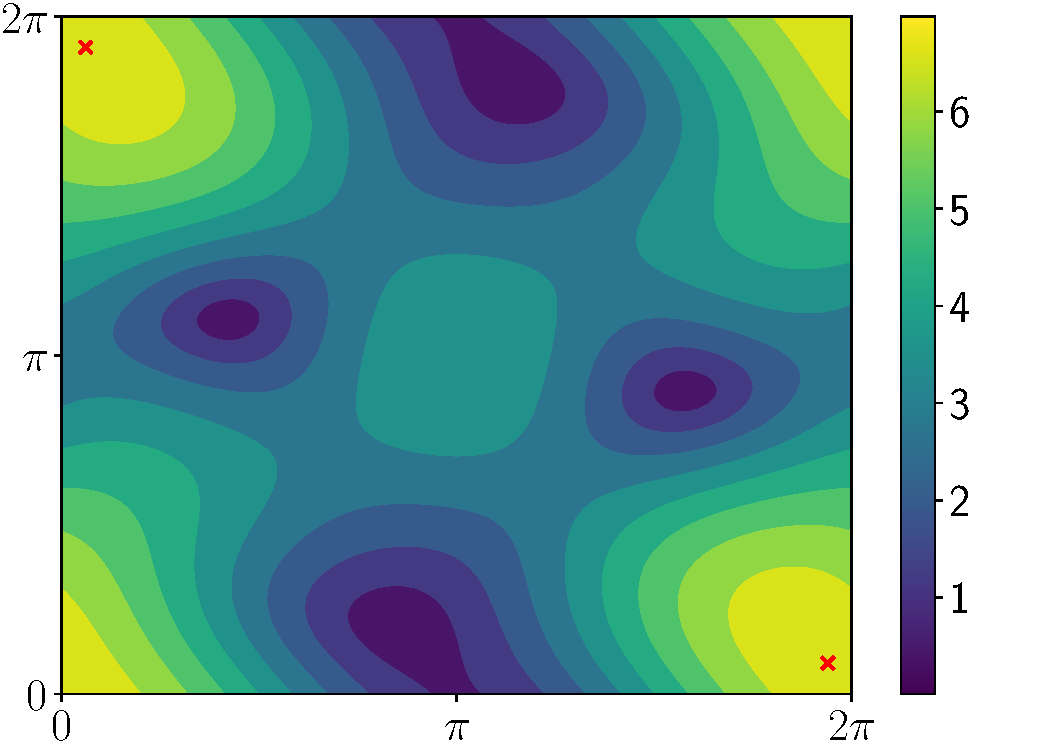
\includegraphics[scale=0.35]{figures/main/ch5-lipschitz_regularization/contour_poly_200_1_1_3.pdf}
    \caption{kernel $1\times3\times3$}
  \end{subfigure}
  \hfill
  \begin{subfigure}[b]{.49\textwidth}
    \centering
    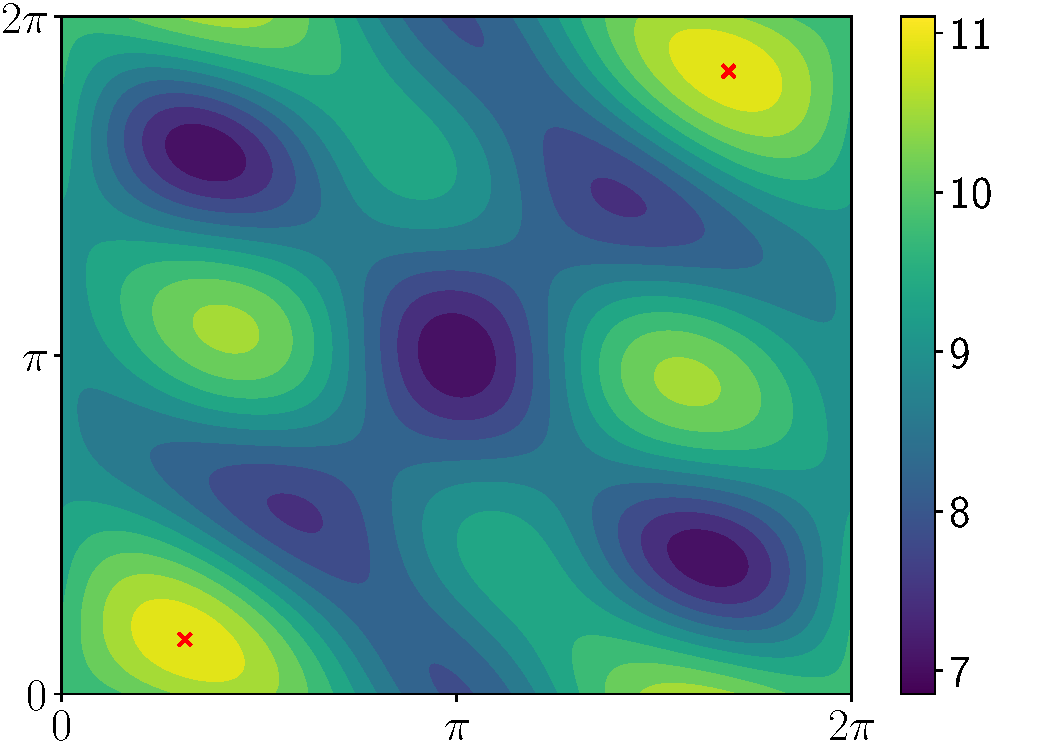
\includegraphics[scale=0.35]{figures/main/ch5-lipschitz_regularization/contour_poly_200_1_9_3.pdf}
    \caption{kernel $9\times3\times3$}
  \end{subfigure}
  \par\bigskip
  \begin{subfigure}[b]{.49\textwidth}
    \centering
    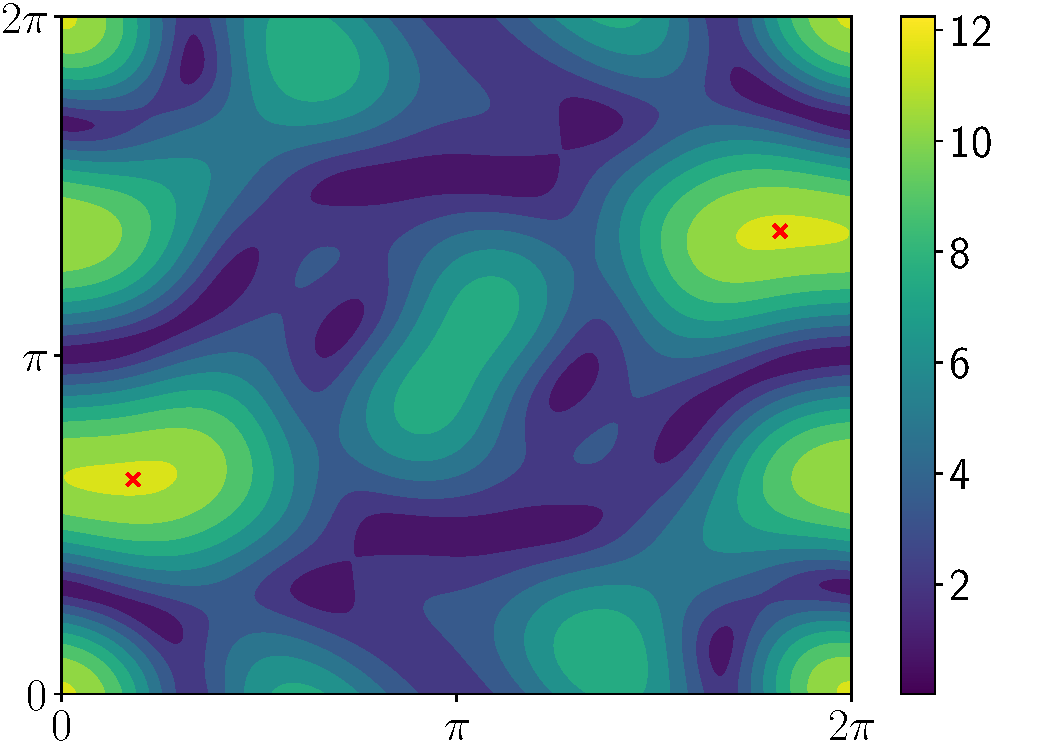
\includegraphics[scale=0.35]{figures/main/ch5-lipschitz_regularization/contour_poly_200_1_1_5.pdf}
    \caption{kernel $1\times5\times5$}
  \end{subfigure}
  \begin{subfigure}[b]{.49\textwidth}
    \centering
    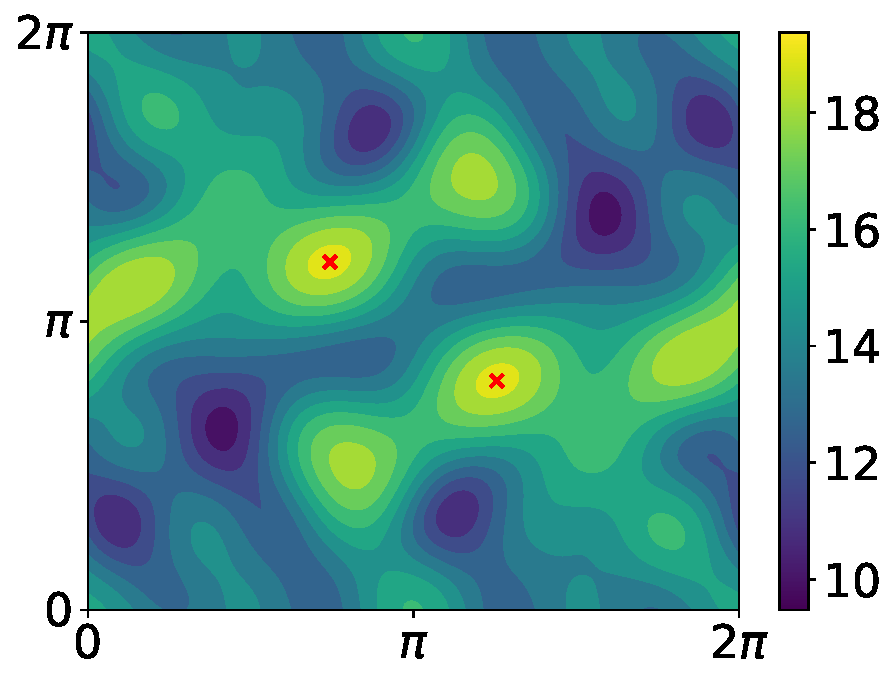
\includegraphics[scale=0.35]{figures/main/ch5-lipschitz_regularization/contour_poly_200_1_9_5.pdf}
    \caption{kernel $9\times5\times5$}
  \end{subfigure}
  \caption{Contour plots of multivariate trigonometric polynomials where the values of the coefficient are the values of a random convolutional kernel. The red dots in the figures represent the maximum modulus of the trigonometric polynomials.}
  \label{figure:contour_plot_trigonometric_polynomials}
\end{figure}%


\begin{algorithm}[htb]
  \begin{algorithmic}[1]
    \Procedure{PolyGrid}{$f, S$}\Comment{polynomial $f$, number of samples $S$}
      \State $\sigma \gets 0$, $\omega_1 \gets 0$, $\epsilon \gets \frac{2\pi}{S}$
      \For{$i=0$ \textbf{to} $S-1$}
        \State $\omega_2 \gets 0$
	\For{$j=0$ \textbf{to} $S-1$}
	  \State $\omega_2 \gets \omega_2 + \epsilon$
	  \State $\sigma \gets \max( \sigma, f(\omega_1, \omega_2))$
	\EndFor
	\State $\omega_1 \gets \omega_1 + \epsilon$
      \EndFor
      \State \textbf{return} $\sigma$ \Comment{approximated maximum modulus of $f$}
    \EndProcedure
  \end{algorithmic}
  \caption{PolyGrid Algorithm}
  \label{algorithm:ch5-polygrid}
\end{algorithm}


To fix the number of samples $S$ in the grid search, we rely on the work of~\cite{pfister2018bounding}, who has analyzed the quality of the approximation depending on $S$.
Following, this work we first define $\Theta_S$, the set of $S$ equidistant sampling points as follows:
\begin{equation}
  \Theta_S \triangleq \left\{ \omega \mid \omega = k \cdot \frac{2\pi}{S} \mbox{ with }  k = 0, \dots, S-1 \right\}.
\end{equation}
Then, for a trigonometric polynomial $f: [0, 2\pi]^2 \rightarrow \Cbb$, we have:
\begin{equation}
  \max_{\omega_1, \omega_2 \in [0,2\pi]^2} \left| f(\omega_1, \omega_2) \right| \leq (1 - \alpha)^{-1} \max_{\omega_1', \omega_2' \in \Theta_S^2} \left| f(\omega_1', \omega_2') \right|,
\end{equation}
where $d$ is the degree of the polynomial and $\alpha = 2d / S$.
For a $3\times3$ kernel which gives a trigonometric polynomial of degree 1, we use $S = 10$ which gives $\alpha = 0.2$.
Using this result, we can now compute $\lipbound$ for a convolution operator with $\cout$ output channels as per \Cref{theorem:bound_sv_stacked_dbt}.
 
% The code to for computing $\lipbound$ with NumPy~\cite{numpy} and PyTorch~\cite{paszke2019pytorch} is publicly available.\footnote{\url{https://github.com/MILES-PSL/upper_bound_lipschitz_convolutional_layers}}.


%%%%%%%%%%%%%%%%%%%%%%%%%%%%%%%%%%%%%%%%%%%%%%%%%%%%%%%%%%%%%%%%%%%%%%%%%%%%%%%%
\subsection{Analysis of the Tightness of the Bound}
\label{subsection:ch2-analysis_of_the_tightness_of_the_bound}
%%%%%%%%%%%%%%%%%%%%%%%%%%%%%%%%%%%%%%%%%%%%%%%%%%%%%%%%%%%%%%%%%%%%%%%%%%%%%%%%

In this section, we study the tightness of the bound with respect to the dimensions of the doubly-block Toeplitz matrices.
For each $n \in \Nbb$, we define the matrix  $\Mmat^{(n)}$ of size $kn^2 \times n^2$ as follows:
\begin{equation}
  \Mmat^{(n)} \triangleq \textstyle \leftmat \Dmat^{(n)\top}(f_1), \dots, \Dmat^{(n)\top}(f_k) \textstyle \rightmat^\top
\end{equation}
where the matrices $\Dmat^{(n)}(f_i)$ are of size $n^2 \times n^2$. 
To analyze the tightness of the bound, we define the function $\Gamma$, which computes the difference between $\lipbound$ and the largest singular value of the function $\Mmat^{(n)}$:
\begin{equation} \label{equation:function_convergence}
  \Gamma(n) = \lipbound(\Kmat_{\Mmat^{(n)}}) - \sigma_1(\Mmat^{(n)})
\end{equation}
where $\Kmat_{\Mmat^{(n)}}$ is the convolution kernel of the convolution defined by the matrix $\Mmat^{(n)}$.

\begin{figure}[ht]
  \centering
  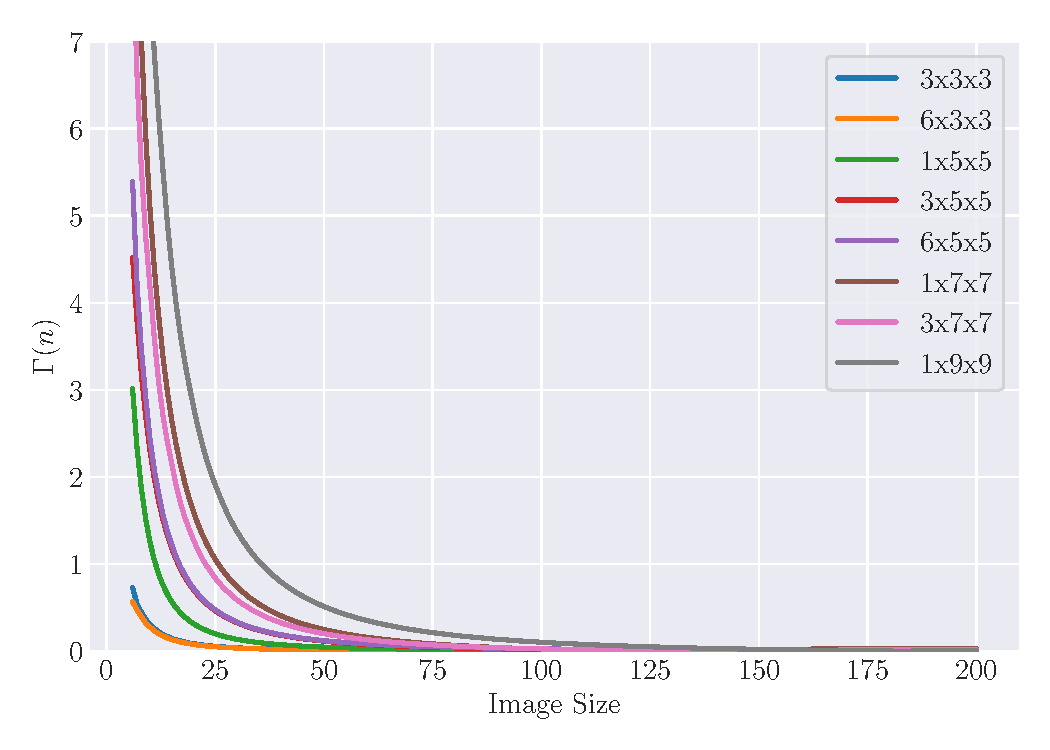
\includegraphics[width=\scalefigure\textwidth]{figures/main/ch5-lipschitz_regularization/convergence_bounds.pdf}
  \caption{Representation of the function $\Gamma(n)$ defined for different kernel size.}
  \label{figure:convergence_bound}
\end{figure}


To compute the exact largest singular value of $\Mmat^{(n)}$ for a specific $n$, we use the Implicitly Restarted Arnoldi Method (IRAM) ~\cite{lehoucq1996deflation} available in SciPy.
The results of this experiment are presented in \Cref{figure:convergence_bound}.
We observe that the difference between the bound and the actual value (approximation gap) quickly decreases as the input size increases.
For an input size of $50$, the approximation gap is as low as $0.012$ using a standard $6\times3\times3$ convolution kernel.
For a larger input size such as ImageNet ($224$), the gap is lower than $4.10^{-4}$.
Therefore $\lipbound$ gives an almost exact value of the largest singular value of the operator matrix for most realistic settings.

%%%%%%%%%%%%%%%%%%%%%%%%%%%%%%%%%%%%%%%%%%%%%%%%%%%%%%%%%%%%%%%%%%%%%%%%%%%%%%%%
\subsection{Comparison of LipBound with State-of-the-Art Approaches}
\label{subsection:ch5-comparison_of_lipbound_with_other_state-of-the-art_approaches}
%%%%%%%%%%%%%%%%%%%%%%%%%%%%%%%%%%%%%%%%%%%%%%%%%%%%%%%%%%%%%%%%%%%%%%%%%%%%%%%%

\begin{table}[ht]
  \centering
  \sisetup{%
    table-align-uncertainty=true,
    separate-uncertainty=true,
    detect-weight=true,
    detect-inline-weight=math
  }
  {\small
  \begin{tabular}%{lrccccrcccc}
    {
      lr
      S[table-format=1.3]@{\,\( \pm \)\,}S[table-format=1.3]
      S[table-format=4.2]@{\,\( \pm \)\,}S[table-format=3.2]
      r
      S[table-format=1.3]@{\,\( \pm \)\,}S[table-format=1.3]
      S[table-format=4.2]@{\,\( \pm \)\,}S[table-format=3.2]
    }
    \toprule
      &   & \multicolumn{4}{c}{\textbf{1x3x3}} &   & \multicolumn{4}{c}{\textbf{32x3x3}} \\
    \cmidrule{3-6} \cmidrule{8-11}
    &   & \multicolumn{2}{c}{\textbf{Ratio}} & \multicolumn{2}{c}{\textbf{Time (ms)}}
    &   & \multicolumn{2}{c}{\textbf{Ratio}} & \multicolumn{2}{c}{\textbf{Time (ms)}} \\
    \midrule
    \citeauthor{sedghi2018singular} &   & 0.431 & 0.042 & 1088 & 251  & & 0.666 & 0.123 & 1729 & 399 \\
    \citeauthor{singla2019bounding} &   & 1.293 & 0.126 & 1.90 & 0.48 & & 1.441 & 0.188 & 1.90 & 0.46 \\
    \citeauthor{farnia2018generalizable} &   & 0.973 & 0.006 & 4.30 & 0.64 & & 0.972 & 0.004 & 4.93 & 0.67 \\
    \midrule
    \midrule
    LipBound &  & 0.992 & 0.012 & 0.49 & 0.05 & & 0.984 & 0.021 & 0.63 & 0.46 \\
    \bottomrule
  \end{tabular}%
  }
  \caption{Comparison of the accuracy of approximation methods for computing an approximation of the largest singular value of a convolutional layer.}
  \label{table:ch5-comparaison_bounds}%
\end{table}



\begin{table}[h]
  \centering
  \sisetup{%
    table-number-alignment=center,
    table-align-uncertainty=true,
    separate-uncertainty=true,
    detect-weight=true,
    detect-inline-weight=math
  }
  \begin{tabular}
    {
      lr
      S[table-format=4.2,table-number-alignment=right]@{\,\( \pm \)\,}S[table-format=2.2,table-number-alignment=left]
      r
      S[table-format=6.2,table-number-alignment=right]@{\,\( \pm \)\,}S[table-format=3.2,table-number-alignment=left]
      r
      S[table-format=1.2]
    }
    \toprule
    \textbf{Network} & & \multicolumn{2}{c}{\textbf{LipBound (ms)}} & & \multicolumn{2}{c}{\textbf{Power Method (ms)}} & & \textbf{Ratio} \\
    \midrule
    AlexNet & & 4.75 & 1.10 & & 38.75 & 2.52 & & 8.14 \\
    \midrule
    ResNet 18 & & 29.88 & 1.73 & & 148.35 & 14.92 & & 4.96 \\
    ResNet 34 & & 54.73 & 3.62 & & 266.85 & 25.35 & & 4.87 \\
    ResNet 50 & & 60.77 & 4.62 & & 467.61 & 36.52 & & 7.69 \\
    ResNet 101 & & 102.72 & 11.53 & & 817.06 & 102.87 & & 7.95 \\
    ResNet 152 & & 158.80 & 20.84 & & 1373.57 & 164.37 & & 8.64 \\
    \midrule
    DenseNet 121 & & 125.55 & 14.59 & &  937.35 &  11.52 & & 7.46 \\
    DenseNet 161 & & 176.11 & 19.13 & & 1292.61 &  30.50 & & 7.33 \\
    DenseNet 169 & & 188.03 & 19.74 & & 1372.62 &  21.16 & & 7.29 \\
    DenseNet 201 & & 281.13 & 23.41 & & 1930.19 & 170.79 & & 6.86 \\
    \midrule
    VGG 11 & & 13.73 & 1.19 & &  81.78 & 4.45 & & 5.95 \\
    VGG 13 & & 14.96 & 1.99 & & 102.04 & 4.20 & & 6.82 \\
    VGG 16 & & 21.92 & 1.94 & & 132.29 & 5.99 & & 6.03 \\
    VGG 19 & & 29.05 & 0.66 & & 162.28 & 4.87 & & 5.58 \\
    \midrule
    WideResnet 50-2 & & 113.28 & 45.44 & & 468.74 & 6.54 & & 4.13 \\
    \midrule
    SqueezeNet 1-0 & & 18.44 & 5.93 & & 222.40 & 25.49 & & 12.05 \\
    SqueezeNet 1-1 & & 18.26 & 6.65 & & 209.80 &  3.59 & & 11.48 \\
    \bottomrule
  \end{tabular}%
  \caption{Efficiency of LipBound computation \vs the Power Method with 10 iterations on full networks.}
  \label{table:ch5-efficiency_lipbound_full_model}%
\end{table}%

In this section we compare our PolyGrid algorithm with the values obtained using alternative approaches.
We consider the 3 alternative techniques by~\citet{sedghi2018singular,singla2019bounding,farnia2018generalizable} which have been described in \Cref{chapter:ch3-related_work}, \Cref{section:ch3-related_work_on_lipschitz_regularization}.

To compare the different approaches, we extracted 20 kernels from a trained model.
For each kernel we construct the corresponding doubly-block Toeplitz matrix and compute its largest singular value.
Then, we compute the ratio between the approximation obtained with the approach in consideration and the exact singular value obtained by SVD, and average the ratios over the 20 kernels.
Thus good approximations result in approximation ratios that are close to 1.
The results of this experiment are presented in \Cref{table:ch5-comparaison_bounds}.
The comparison has been made on a Tesla V100 GPU.
The time was computed with the PyTorch CUDA profiler and we warmed up the GPU before starting the timer.

The method introduced by~\citet{sedghi2018singular} and presented in~\Cref{subsection:ch3-singular_values_of_convolutional_layers} computes the largest singular value of convolutional layers based on doubly-block circulant matrices.
Doubly-block circulant matrices perform a convolution with a ``wrapping around'' operation which do not correspond to the more general setting.
We can see in \Cref{table:ch5-comparaison_bounds} that the value is off by an important margin.
This technique is also computationally expensive as it requires computing the SVD of $n^2$ small matrices where $n$ is the size of inputs.
\citet{singla2019bounding} have shown that the singular value of the reshape kernel is a bound on the largest singular value of the convolution layer.
Their approach is very efficient but the approximation is loose and overestimate the real value.
As said previously, the power method provides a good approximation at the expense of the efficiency.
We also compare our approach to the power method with 10 iterations from ~\citet{farnia2018generalizable} (see~\Cref{algorithm:ch3-power_method_generic}).
The results show that our proposed technique: PolyGrid algorithm can get the best of both worlds.
It achieves a near perfect accuracy while being very efficient to compute.


We also compare in~\Cref{table:ch5-efficiency_lipbound_full_model} our method against the power method of~\citet{farnia2018generalizable} on the following convolutional architectures: AlexNet \cite{krizhevsky2012imagenet}, ResNet \cite{he2016deep}, DenseNet \cite{huang2017densely}, VGG \cite{simonyan2014very}, WideResnet \cite{zagoruyko2016wide}, SqueezeNet \cite{iandola2016squeezenet}.
During training, Lipbound or the power method need to be computed for every layer of the network and the computation time is dependent on the architecture of the network, for example, the size of the activations or the size of the kernels.
\Cref{table:ch5-efficiency_lipbound_full_model} shows that for full networks Lipbound is systematically faster than the power method by a factor up to 12.
This demonstrates the scalability of our method.




%%%%%%%%%%%%%%%%%%%%%%%%%%%%%%%%%%%%%%%%%%%%%%%%%%%%%%%%%%%%%%%%%%%%%%%%%%%%%%%%
\section{Lipschitz Regularization for Adversarial Robustness}
\label{section:ch5-lipschitz_regularization_for_adversarial_robustness}
%%%%%%%%%%%%%%%%%%%%%%%%%%%%%%%%%%%%%%%%%%%%%%%%%%%%%%%%%%%%%%%%%%%%%%%%%%%%%%%%



One promising application of Lipschitz regularization is in the area of adversarial robustness.
Empirical techniques to improve robustness against adversarial examples such as Adversarial Training only impact the training data,  and often show poor generalization capabilities~\cite{schmidt2018adversarially}.
\citet{farnia2018generalizable} have shown that the adversarial generalization error depends on the Lipschitz constant of the network, which suggests that the adversarial test error can be improved by applying Lipschitz regularization in addition to adversarial training.

In this section, we illustrate the usefulness of LipBound by training a state-of-the-art Wide ResNet architecture~\citep{zagoruyko2016wide} with Lipschitz regularization and adversarial training.
Our regularization scheme is inspired by the one used by \citet{yoshida2017spectral} but instead of using the power method, we use our \textbf{PolyGrid} algorithm presented in~\Cref{subsection:ch5-computing_the_maximum_modulus_of_a_trigonometric_polynomial} which efficiently computes an upper bound on the largest singular value of convolutional layers.

We introduce the \textbf{AT+LipReg} loss to combine Adversarial Training and our Lipschitz regularization scheme in which layers with a large Lipschitz constant are penalized.
We consider a neural network $N_\Omega : \Xset \rightarrow \Yset$ with $\depth$ layers $\phi^{(1)}_{\Wmat^{(1)}, \bvec^{(1)}}, \dots, \phi^{(\depth)}_{\Wmat^{(\depth)}, \bvec^{(\depth)}}$ where $\Wmat^{(1)}, \dots, \Wmat^{(\depth)}$ are the weight matrices and $\Omega$ is the union of all the parameters as defined in~\Cref{definition:ch2-neural_networks}.
Given a distribution $\Dset$ over $\Xset \times \Yset$, we can train the parameters of the network by minimizing the AT+LipReg loss as follows:
\begin{equation} \label{equation:ch5-obj_function}
  \min_{\Omega} \Ebb_{\xvec,y \sim \Dset} \left[ L(N_\Omega(\xvec + \adv^{\text{adv}}_\Omega(\xvec)), y) + r(\Omega) \right]
\end{equation}
where $L$ is the cross-entropy loss function, $\adv^{\text{adv}}_\Omega(\xvec)$ is an adversarial perturbation following the loss maximization strategy presented in~\Cref{subsubsection:ch2-adversarial_attacks} and the regularization function $r$ is defined as follows:
\begin{equation}
  r(\Omega) =  C_1 \underbrace{\sum_{(\Wmat, \bvec) \in \Omega} \left( \norm{\Wmat}_\fro + \norm{\bvec}_2 \right)}_{
  \text{Tikhonov regularization}} + C_2 \underbrace{\vphantom{\sum_{(\Wmat, \bvec) \in \Omega}} \sum_{i=1}^{\depth-1} \log\left(\lipbound\left(\Kmat_{\Wmat^{(i)}}\right)\right)}_{\text{Lipschitz regularization}} 
\end{equation}
where $C_1$, $C_2$ are two user-defined hyper-parameters.
Note that regularizing the sum of logs is equivalent to regularizing the product of all the $\lipbound$ which is an upper bound on the global Lipschitz constant.
In practice, we also include the upper bound on the Lipschitz of the batch normalization because we can compute it very efficiently (see C.4.1 of ~\citet{tsuzuku2018lipschitz}) but we omit the last fully connected layer.

In this section, we compare the robustness of Adversarial Training~\cite{goodfellow2014explaining, madry2018towards} against the combination of Adversarial Training and Lipschitz regularization.
To regularize the Lipschitz constant of the network, we use the objective function defined in Equation~\ref{equation:ch5-obj_function}.
We train Lipschitz regularized neural networks with LipBound (see~\Cref{theorem:ch5-bound_max_sv_convolution}) implemented with PolyGrid (see~\Cref{algorithm:ch5-polygrid}) (AT+LipBound) with $S = 10$ or with the specific power method for convolutions introduced by~\citet{farnia2018generalizable} with 10 iterations (AT+PM).

Table~\ref{table:ch5-cifar_robustness} shows the gain in robustness against strong adversarial attacks across different datasets.
We can observe that both AT+LipBound and AT+PM offer a better defense against adversarial attacks and that AT+LipBound offers a further improvement over the Power Method.
The \Cref{figure:ch5-attacks_pgd,figure:ch5-attacks_cw} shows the Accuracy under attack with different number of iterations.
Table~\ref{table:ch5-results_imagenet_dataset} presents our results on the ImageNet Dataset.
First, we can observe that the networks AT+LipReg offers a better generalization than with standalone Adversarial Training.
Secondly, we can observe the gain in robustness against strong adversarial attacks.
Network trained with Lipschitz regularization and Adversarial Training offer a consistent increase in robustness across $\ell_\infty$ and $\ell_2$ attacks with different $\epsilon$ value.
We can also note that increasing the regularization lead to an increase in generalization and robustness.

\afterpage{
\begin{figure}[p!]
   \centering
   \begin{subfigure}[b]{\textwidth}
     \centering
     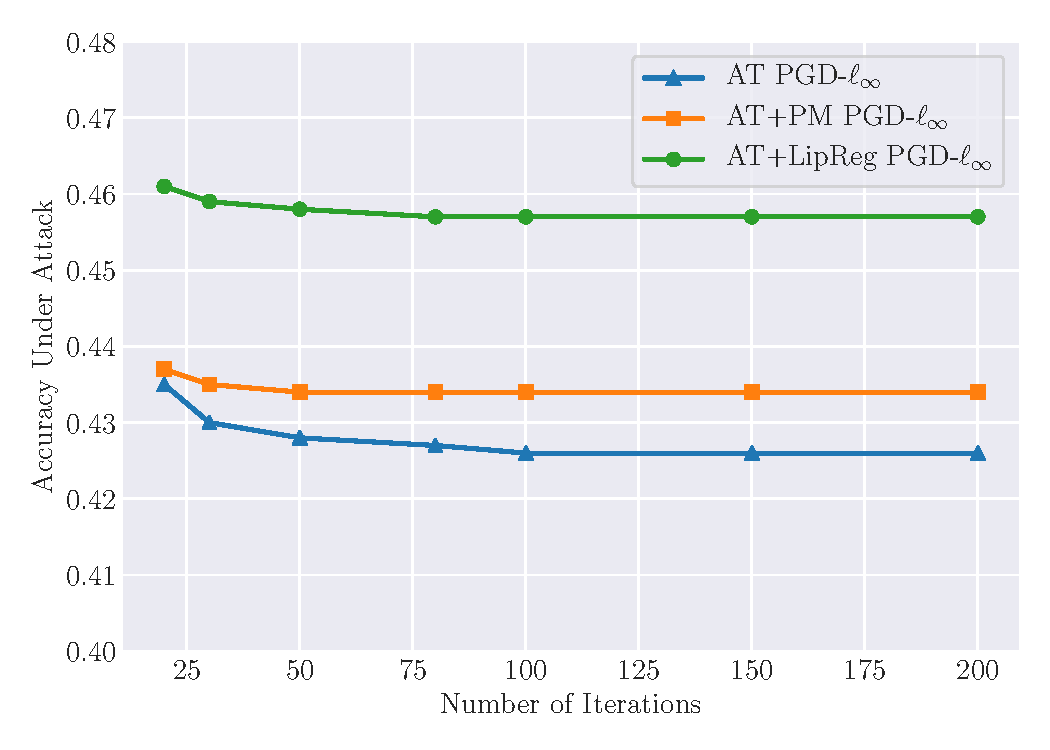
\includegraphics[width=\scalefigure\textwidth]{figures/main/ch5-lipschitz_regularization/attacks_iter_pgd.pdf}
     \caption{Robustness against $\ell_\infty$ attacks for different classifiers trained with Adversarial Training given the number of iterations.}
     \label{figure:ch5-attacks_pgd}
   \end{subfigure}
   ~\\[1cm]
   \begin{subfigure}[b]{\textwidth}
     \centering
     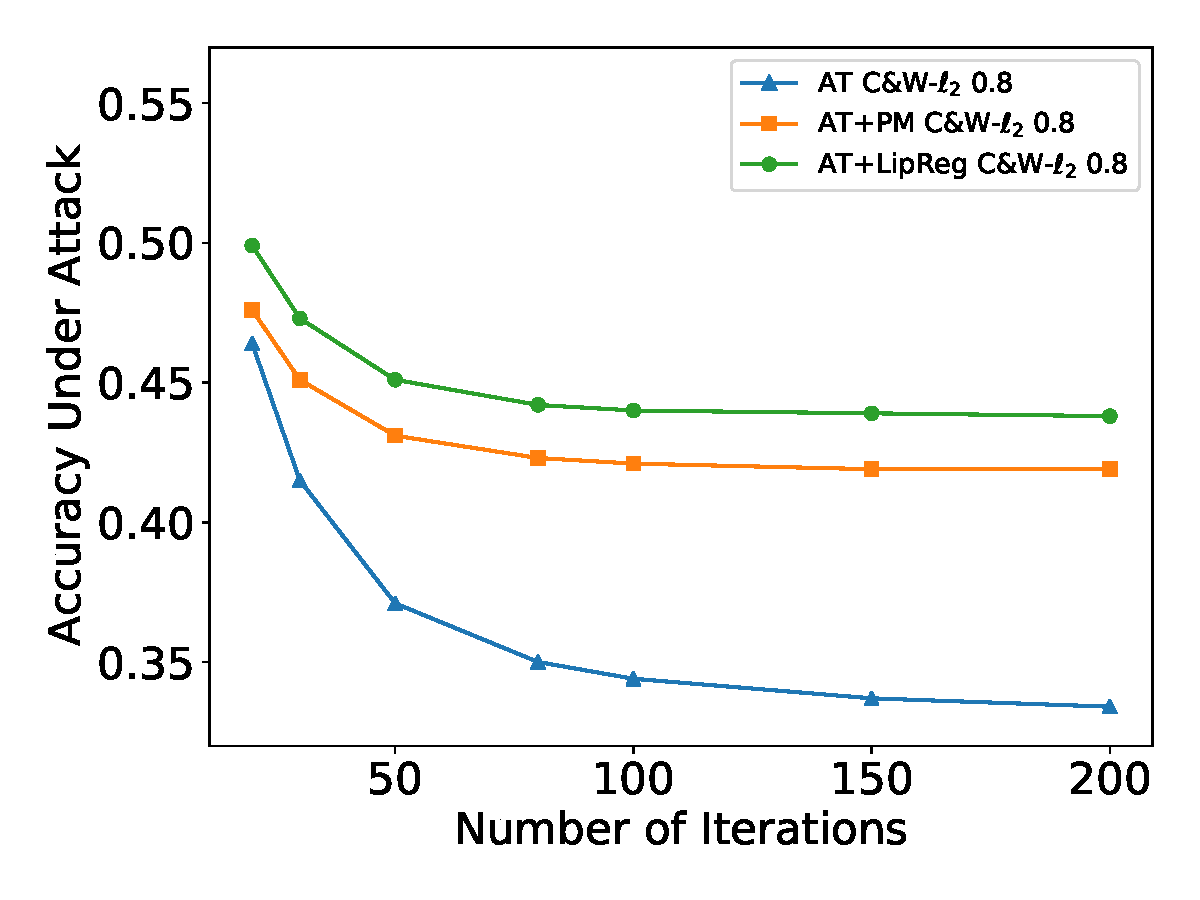
\includegraphics[width=\scalefigure\textwidth]{figures/main/ch5-lipschitz_regularization/attacks_iter_cw.pdf}
     \caption{Robustness against $\ell_\infty$ attacks for different classifiers trained with Adversarial Training given the number of iterations.}
     \label{figure:ch5-attacks_cw}
   \end{subfigure}
   ~\\[1cm]
   \caption{Accuracy under attack on CIFAR10 test set with $\ell_\infty$ and $\ell_2$ attacks for several classifiers trained with Adversarial Training given the number of iterations.}
\end{figure}
\clearpage
}


\afterpage{
\begin{figure}[p!]
   \centering
   \begin{subfigure}[b]{\textwidth}
     \centering
     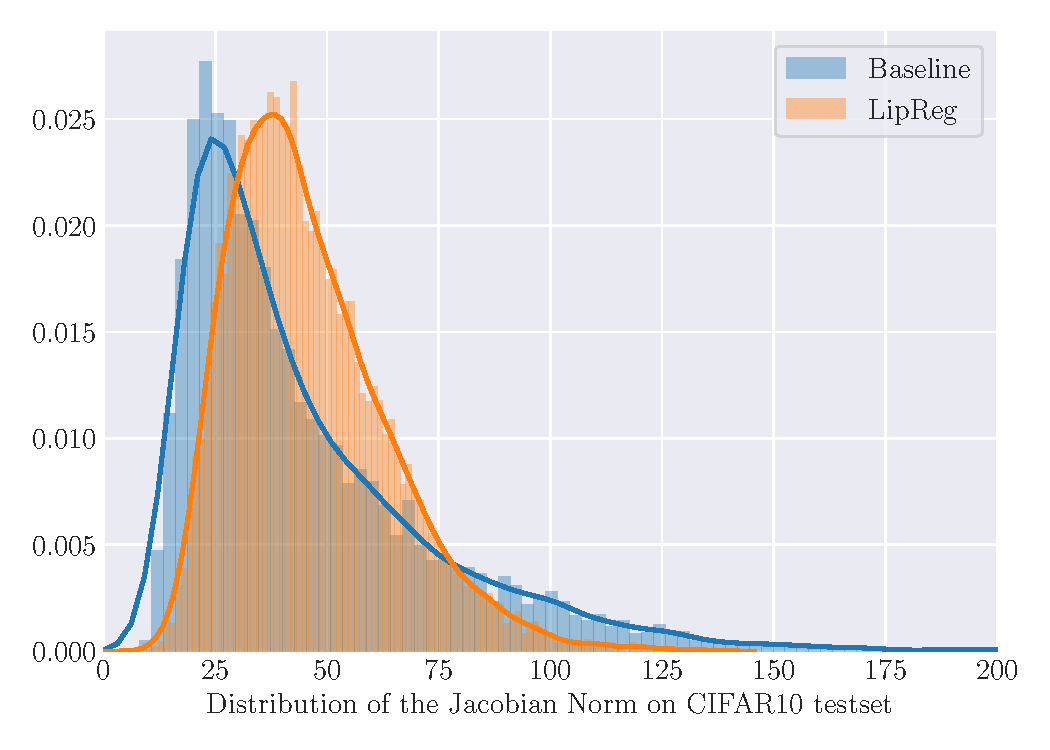
\includegraphics[width=\scalefigure\textwidth]{figures/main/ch5-lipschitz_regularization/jacobian_distribution_v1.pdf}
     \caption{Comparison of the distribution of the norm of the Jacobian of the baseline model against the model trained with Lipschitz regularization.}
     \label{figure:ch5-jacobian_distribution_v1}
   \end{subfigure}
   ~\\[1cm]
   \begin{subfigure}[b]{\textwidth}
      \centering
      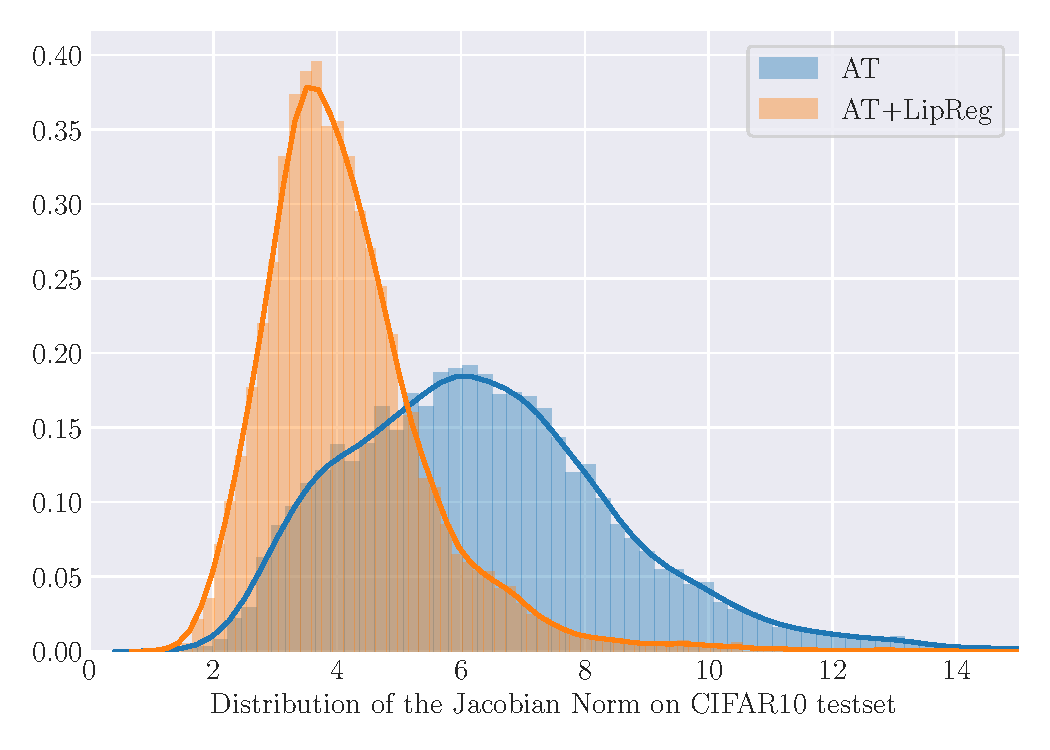
\includegraphics[width=\scalefigure\textwidth]{figures/main/ch5-lipschitz_regularization/jacobian_distribution_v2.pdf}
      \caption{Comparison of the distribution of the norm of the Jacobian of the model trained with Adversarial training against the model trained with Adversarial training and Lipschitz regularization.}
      \label{figure:ch5-jacobian_distribution_v2}
   \end{subfigure}
   ~\\[1cm]
   \caption{Distribution of the norm of the Jacobian matrix with respect to the CIFAR10 test set from a Wide Resnet trained with different schemes.} 
\end{figure}
\clearpage
}


Finally, we also conducted an experiment to study the impact of the regularization on the gradients of the whole network by measuring the norm of the Jacobian matrix, averaged over the inputs from the test set.
The results of this experiment are presented in~\Cref{figure:ch5-jacobian_distribution_v1} and show more concentrated gradients with  Lipschitz regularization, which is the expected effect.
Although Lipschitz regularization is not a Jacobian regularization, we can observe a clear shift in the distribution.
This suggests that our method does not only work layer-wise, but also at the level of the entire network.
A second experiment, using Adversarial Training, presented in~\Cref{figure:ch5-jacobian_distribution_v2} demonstrates that the effect is even stronger when the two techniques are combined together.
This corroborates the work by~\citet{farnia2018generalizable}.
It also demonstrates that Lipschitz regularization and Adversarial Training (or other Jacobian regularization techniques) are complementary.
Hence they offer an increased robustness to adversarial attacks as demonstrated above.


\begin{table}[t]
  \sisetup{%
    table-align-uncertainty=true,
    separate-uncertainty=true,
    detect-weight=true,
    detect-inline-weight=math
  }
  \centering
  \begin{subfigure}[b]{\textwidth}
    \begin{tabular}
      {
	l
        S[table-format=1.3]@{\,\( \pm \)\,}S[table-format=1.3]
        S[table-format=1.3]@{\,\( \pm \)\,}S[table-format=1.3]
        S[table-format=1.3]@{\,\( \pm \)\,}S[table-format=1.3]
        S[table-format=1.3]@{\,\( \pm \)\,}S[table-format=1.3]
      }
      \toprule
      \textbf{Model} & \multicolumn{2}{c}{\textbf{Accuracy}} & \multicolumn{2}{c}{\textbf{PGD-$\ell_\infty$}}
      & \multicolumn{2}{c}{\textbf{C\&W-$\ell_2$ 0.6}} & \multicolumn{2}{c}{\textbf{C\&W-$\ell_2$ 0.8}} \\
      \midrule
      \textbf{Baseline} & \textbf{0.953} & 0.001 & 0.000 & 0.000 & 0.002 & 0.000 & 0.000 & 0.000 \\
      \textbf{AT}       & 0.864 & 0.001 & 0.426 & 0.000 & 0.477 & 0.000 & 0.334 & 0.000 \\
      \textbf{AT+PM}    & 0.788 & 0.010 & 0.434 & 0.007 & 0.521 & 0.005 & 0.419 & 0.003 \\
      \textbf{AT+LipReg} & 0.808 & 0.022 & \textbf{0.457} & 0.002 & \textbf{0.547} & 0.022 & \textbf{0.438} & 0.020 \\
      \bottomrule
    \end{tabular}%
    \caption{Results on CIFAR10 dataset}
    \label{subfigure:ch5-results_cifar10_data}
  \end{subfigure}
  \par\bigskip
  \begin{subfigure}[b]{\textwidth}
    \begin{tabular}
      {
	l
        S[table-format=1.3]@{\,\( \pm \)\,}S[table-format=1.3]
        S[table-format=1.3]@{\,\( \pm \)\,}S[table-format=1.3]
        S[table-format=1.3]@{\,\( \pm \)\,}S[table-format=1.3]
        S[table-format=1.3]@{\,\( \pm \)\,}S[table-format=1.3]
      }
      \toprule
      \textbf{Model} & \multicolumn{2}{c}{\textbf{Accuracy}} & \multicolumn{2}{c}{\textbf{PGD-$\ell_\infty$}}
      & \multicolumn{2}{c}{\textbf{C\&W-$\ell_2$ 0.6}} & \multicolumn{2}{c}{\textbf{C\&W-$\ell_2$ 0.8}} \\
      \midrule
      \textbf{Baseline} & \textbf{0.792} & 0.000  & 0.000 & 0.000  & 0.001 & 0.000  & 0.000 & 0.000 \\
      \textbf{AT} & 0.591 & 0.000  & 0.199 & 0.000  & 0.263 & 0.000  & 0.183 & 0.000 \\
      \textbf{AT+LipReg} & 0.552 & 0.019  & \textbf{0.215} & 0.004  & \textbf{0.294} & 0.010  & \textbf{0.226} & 0.008  \\
      \bottomrule
    \end{tabular}%
    \caption{Results on CIFAR100 dataset}
    \label{subfigure:ch5-results_cifar100_data}
  \end{subfigure}
  \caption{Accuracy under $\ell_2$ and $\ell_\infty$ attacks of different training schemes on CIFAR10/100 datasets.} 
% We compare vanilla Adversarial Training with the combination of Lipschitz regularization and Adversarial Training. We also compare the effectiveness of the power method by~\citet{farnia2018generalizable} and $\lipbound$. We fix the parameter $\lambda_2$ from \Cref{equation:ch5-obj_function}) to $0.008$ for AT+PM and AT+LipReg. It has been chosen from a grid search among 10 values. The attacks are computed with 200 iterations. }
  \label{table:ch5-cifar_robustness}%
\end{table}%


\begin{table}[t]
  \centering
  \tabcolsep=1.9mm
  {\small
  \begin{tabular}{
    lc
    c
    cc
    c
    ccc
  }
    \toprule
    \multicolumn{1}{c}{\multirow{2}[4]{*}{\textbf{Model}}} & \multicolumn{1}{c}{\multirow{2}[4]{*}{\textbf{Natural}}} &  
    & \multicolumn{2}{c}{\textbf{PGD}-$\ell_\infty$} &   & \multicolumn{3}{c}{\textbf{C\&W}-$\ell_2$} \\
    \cmidrule{4-5}\cmidrule{7-9} 
    &  &  & \multicolumn{1}{c}{0.02} & \multicolumn{1}{c}{0.031} &   & \multicolumn{1}{c}{1.00} & \multicolumn{1}{c}{2.00} & \multicolumn{1}{c}{3.00} \\
    \midrule
    \textbf{Baseline} \cite{he2016deep} & \textbf{0.782} & & 0.000 & 0.000 & & 0.000 & 0.000 & 0.000 \\
    \textbf{AT} & 0.509 &   & 0.251 & 0.118 &   & 0.307 & 0.168 & 0.099 \\
    \textbf{AT+LipReg} ($C_2 = 0.0006$) & \textbf{0.515} &   & \textbf{0.255} & \textbf{0.121} &   & \textbf{0.316} & \textbf{0.177} & \textbf{0.105} \\
    \textbf{AT+LipReg} ($C_2 = 0.0010$) & \textbf{0.519} &   & \textbf{0.259} & \textbf{0.123} &   & \textbf{0.338} & \textbf{0.204} & \textbf{0.129} \\
    \bottomrule
  \end{tabular}%
  }
  % \caption{This table shows the accuracy and accuracy under $\ell_2$ and $\ell_\infty$ attack of ImageNet dataset. We compare Adversarial Training with the combination of Lipschitz regularization and Adversarial Training \cite{madry2018towards}. }
  \caption{Natural accuracy and accuracy under $\ell_2$ and $\ell_\infty$ attacks of different training schemes on the ImageNet dataset.} 
  \label{table:ch5-results_imagenet_dataset}
\end{table}%





\paragraph{Experimental Settings CIFAR10/100 Dataset.}
For all our experiments, we use the Wide ResNet architecture introduced by~\citet{zagoruyko2016wide} to train our classifiers.
We use Wide Resnet networks with 28 layers and a width factor of 10.
We train our networks for 200 epochs with a batch size of $200$.
We use Stochastic Gradient Descent with a momentum of $0.9$, an initial learning rate of $0.1$ with exponential decay of 0.1 (MultiStepLR gamma = 0.1) after the epochs $60$, $120$ and $160$.
For Adversarial Training ~\cite{madry2018towards}, we use Projected Gradient Descent with an $\epsilon = 8/255 (\approx 0.031)$, a step size of $\epsilon/5 (\approx 0.0062)$ and 10 iterations, we use a random initialization but run the attack only once.
To evaluate the robustness of our classifiers, we rigorously followed the experimental protocol proposed by~\citet{carlini2019evaluating,tramer2020adaptive}.
More precisely, as an $\ell_\infty$ attack, we use PGD with the same parameters ($\epsilon = 8/255$, a step size of $\epsilon/5$) but we increase the number of iterations up to 200 with 10 restarts.
For each image, we select the perturbation that maximizes the loss among all the iterations and the 10 restarts.
As $\ell_2$ attacks, we use a bounded version of the~\citet{carlini2017towards} attack.
We choose $0.6$ and $0.8$ as bounds for the $\ell_2$ perturbation.
Note that the $\ell_2$ ball with a radius of $0.8$ has approximately the same volume as the $\ell_\infty$ ball with a radius of $0.031$ for the dimensionality of CIFAR10/100.


\paragraph{Experimental Settings for ImageNet Dataset.}
For all our experiments, we use the Resnet-101 architecture \cite{he2016deep}.
We have used Stochastic Gradient Descent with a momentum of $0.9$, a weight decay of $0.0001$, label smoothing of $0.1$, an initial learning rate of $0.1$ with exponential decay of $0.1$ (MultiStepLR gamma = $0.1$) after the epochs $30$ and $60$.
We have used Exponential Moving Average over the weights with a decay of $0.999$.
We have trained our networks for 80 epochs with a batch size of $4096$.
For Adversarial Training, we have used PGD with 5 iterations, $\epsilon = 8/255 (\approx 0.031)$ and a step size of $\epsilon/5 (\approx 0.0062)$.
To evaluate the robustness of our classifiers on ImageNet Dataset, we have used an $\ell_\infty$ and an $\ell_2$ attacks.
More precisely, as an $\ell_\infty$ attack, we use PGD with an epsilon of 0.02 and 0.031, a step size of $\epsilon/5$) with a number of iterations to 30 with 5 restarts.
For each image, we select the perturbation that maximizes the loss among all the iterations and the 10 restarts.
As $\ell_2$ attacks, we use a bounded version of the~\citet{carlini2017towards} attack.
We have used $1$, $2$ and $3$ as bounds for the $\ell_2$ perturbation.


%%%%%%%%%%%%%%%%%%%%%%%%%%%%%%%%%%%%%%%%%%%%%%%%%%%%%%%%%%%%%%%%%%%%%%%%%%%%%%%%
\section{Concluding Remarks}
\label{section:ch5-concluding_remarks}
%%%%%%%%%%%%%%%%%%%%%%%%%%%%%%%%%%%%%%%%%%%%%%%%%%%%%%%%%%%%%%%%%%%%%%%%%%%%%%%%

In this chapter, we introduced a new bound on the Lipschitz constant of convolutional layers that is both accurate and efficient to compute.
We used this bound to regularize the Lipschitz constant of neural networks and demonstrated its computational efficiency in training large neural networks with a regularized Lipschitz constant.
As an illustrative example, we combined our bound with adversarial training, and showed that this increases the robustness of the trained networks to  adversarial attacks.
The scope of our results goes beyond this application and can be used in a wide variety of settings, for example, to stabilize the training of Generative Adversarial Networks (GANs) and invertible networks, or to improve generalization capabilities of classifiers.

